% SOITraCS Final Report - IEEE Conference Format
\documentclass[conference]{IEEEtran}

% Packages
\usepackage{amsmath,amssymb,amsfonts}
\usepackage{algorithmic}
\usepackage{graphicx}
\usepackage{textcomp}
\usepackage{xcolor}
\usepackage{booktabs}
\usepackage{multirow}
\usepackage{array}
\usepackage{url}
\usepackage{balance}

% Hyperref for clickable links
\usepackage[colorlinks=true,linkcolor=blue,citecolor=blue,urlcolor=blue]{hyperref}
\usepackage{cite}

% TikZ for architecture diagram
\usepackage{tikz}
\usetikzlibrary{shapes, arrows.meta, positioning, fit}

% Custom colors
\definecolor{SOITraCSTeal}{RGB}{0, 128, 128}

\begin{document}

\title{SOITraCS: A Multi-Algorithm Framework for\\Self-Organizing Intelligent Traffic Control}

\author{
\IEEEauthorblockN{Cojocariu Raul}
\IEEEauthorblockA{
Department of Artificial Intelligence\\
Politehnica University of Bucharest\\
Bucharest, Romania}
\and
\IEEEauthorblockN{Patrascu Adrian}
\IEEEauthorblockA{
Department of Artificial Intelligence\\
Politehnica University of Bucharest\\
Bucharest, Romania}
}

\maketitle

\begin{abstract}
Adaptive traffic signal control remains a challenging problem due to the stochastic nature of traffic flow and the need for real-time responsiveness. This paper presents SOITraCS (\textbf{S}elf-\textbf{O}rganizing \textbf{I}ntelligent \textbf{Tra}ffic \textbf{C}ontrol \textbf{S}ystems), a simulation framework that integrates eight self-organizing algorithms: Cellular Automata for microscopic vehicle dynamics, Self-Organizing Traffic Lights for decentralized signal control, Ant Colony Optimization for dynamic routing, Particle Swarm Optimization for parameter tuning, Self-Organizing Maps for traffic pattern recognition, Multi-Agent Reinforcement Learning for adaptive coordination, Enhanced MARL with Double Q-learning for improved value estimation, and Pressure-Based Control for queue balancing. Unlike approaches that study these methods in isolation, SOITraCS employs an event-driven architecture that enables inter-algorithm communication through a publish/subscribe mechanism. Experiments across 480 simulation runs indicate that the integrated system reduces average vehicle delay by 44.7\% compared to fixed-timing baselines. Ablation analysis reveals that while SOTL and ACO each contribute roughly 30\% improvement independently, the pattern recognition component (SOM) provides an additional 11.3\% benefit through its role as an integration enabler rather than a direct controller.
\end{abstract}

\begin{IEEEkeywords}
self-organizing systems, traffic signal control, ant colony optimization, multi-agent reinforcement learning, cellular automata
\end{IEEEkeywords}

\section{Introduction}

As a consequence of urbanization and population growth, transportation demand continues to rise in metropolitan areas worldwide. The resulting congestion carries substantial economic costs---the Texas A\&M Transportation Institute estimates that American commuters lose an average of 54 hours annually to traffic delays \cite{schrank2019}---while also contributing to environmental degradation through increased vehicle emissions.

Early traffic control systems addressed this challenge through fixed-timing signal controllers, which operate on predetermined schedules calibrated for average demand patterns. While straightforward to deploy and maintain, such systems cannot respond to the inherent variability of real traffic: rush-hour surges, incidents, weather disruptions, and special events all generate demand patterns that static controllers fail to accommodate. This limitation has motivated decades of research into adaptive control methods.

Self-organizing approaches represent one promising direction. Unlike centralized optimization schemes that require global state information and substantial computational resources, self-organizing systems rely on local interactions between autonomous components \cite{gershenson2005}. Individual intersections or vehicles make decisions based on immediate conditions, and coordination emerges from their collective dynamics rather than explicit programming. This paradigm offers natural scalability, since adding network elements requires no reconfiguration, and inherent fault tolerance, as the system continues functioning when individual components fail.

The literature contains numerous self-organizing methods applicable to traffic: cellular automata for vehicle dynamics \cite{nagel1992cellular}, threshold-based signal switching \cite{cools2013sotl}, pheromone-guided routing \cite{dorigo1997aco}, swarm-based parameter optimization \cite{kennedy1995pso}, and multi-agent reinforcement learning \cite{chu2019marl}. However, most studies examine these techniques in isolation. Less attention has been paid to how multiple self-organizing algorithms might interact when deployed together---whether they interfere, complement each other, or produce emergent synergies.

This paper describes SOITraCS, a framework designed to investigate such interactions. The system integrates six algorithms within an event-driven architecture where components communicate through typed messages rather than direct coupling. We conduct ablation experiments to quantify individual contributions and identify cases where algorithm combinations yield benefits exceeding their independent effects.

The remainder of this paper proceeds as follows. Section~II surveys related work on self-organizing traffic control. Section~III describes the system architecture and algorithm implementations. Section~IV details the experimental methodology, and Section~V presents results. Section~VI discusses findings and concludes.

\section{Related Work}

\subsection{Microscopic Traffic Simulation}

Cellular automaton models provide a computationally efficient approach to microscopic traffic simulation. Nagel and Schreckenberg \cite{nagel1992cellular} introduced a model where vehicles occupy discrete cells and update their positions according to four rules: acceleration toward a maximum speed, deceleration to avoid collisions, stochastic slowdown, and movement. Despite its simplicity, this formulation reproduces empirically observed phenomena including spontaneous jam formation and stop-and-go waves. Subsequent work extended the model to multi-lane roads \cite{rickert1996} and intersection dynamics.

\subsection{Decentralized Signal Control}

Cools, Gershenson, and D'Hooghe \cite{cools2013sotl} proposed Self-Organizing Traffic Lights (SOTL), where each intersection monitors approaching vehicle queues and switches phases when counts exceed configurable thresholds. Additional mechanisms prevent splitting platoons and enforce minimum green times. Simulation studies demonstrated that SOTL matches or exceeds globally optimized controllers in many scenarios, despite using only local information. Gershenson \cite{gershenson2005} analyzed how ``green waves''---corridors of synchronized signals---emerge from purely local switching rules without explicit coordination.

\subsection{Swarm Intelligence}

Ant Colony Optimization, introduced by Dorigo and Gambardella \cite{dorigo1997aco}, models collective behavior in ant colonies where pheromone trails guide foraging. Applied to routing, successful paths accumulate pheromone while evaporation removes outdated information, naturally biasing subsequent travelers toward faster routes. D'Acierno et al. \cite{dacierno2006} demonstrated ACO's effectiveness for dynamic vehicle routing in congested networks.

Particle Swarm Optimization \cite{kennedy1995pso} addresses continuous parameter tuning through simulated swarm dynamics. Particles representing candidate solutions move through the parameter space, influenced by their own best-found positions and the swarm's global best. Garcia-Nieto et al. \cite{garcianieto2012} applied PSO to signal timing optimization, treating phase durations as continuous variables.

\subsection{Learning-Based Approaches}

Kohonen's Self-Organizing Maps \cite{kohonen1990som} provide unsupervised clustering while preserving topological relationships---similar inputs map to adjacent neurons. For traffic applications, SOMs can classify operational states (normal flow, congestion, incidents) and trigger appropriate responses.

Multi-agent reinforcement learning has attracted considerable recent interest. Chu et al. \cite{chu2019marl} developed a scalable approach where each intersection learns an independent policy while sharing experiences across the network. Wei et al. \cite{wei2019} survey the growing literature on RL-based signal control, noting both successes and remaining challenges regarding sample efficiency and transfer across network topologies.

\subsection{Integration Gap}

While each approach above has been studied extensively, few works examine how multiple self-organizing methods interact within a unified system. Most comparative studies evaluate algorithms independently against common baselines rather than investigating potential synergies or interference effects. SOITraCS addresses this gap through an architecture that enables systematic study of algorithm combinations.

\section{System Design}

\subsection{Architecture Overview}

SOITraCS adopts a three-layer design with publish/subscribe communication (Fig.~\ref{fig:architecture}). The core layer provides simulation infrastructure: a road network represented as a directed graph, traffic signal state machines, and vehicle entities. The algorithm layer contains eight self-organizing modules, each subscribing to relevant events and publishing its outputs. The presentation layer handles visualization and user interaction.

\begin{figure}[t]
\centering
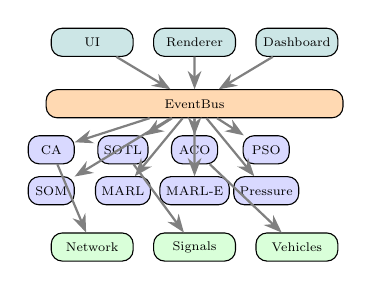
\begin{tikzpicture}[
    scale=0.65, transform shape,
    box/.style={rectangle, draw, rounded corners, minimum width=1.6cm, minimum height=0.55cm, align=center, font=\scriptsize},
    algobox/.style={rectangle, draw, rounded corners, minimum width=0.9cm, minimum height=0.55cm, align=center, font=\scriptsize},
    arrow/.style={-{Stealth}, thick, gray}
]
    \node[box, fill=SOITraCSTeal!20] (ui) at (0.8, 2.4) {UI};
    \node[box, fill=SOITraCSTeal!20] (render) at (2.8, 2.4) {Renderer};
    \node[box, fill=SOITraCSTeal!20] (dash) at (4.8, 2.4) {Dashboard};
    \node[box, fill=orange!30, minimum width=5.8cm] (bus) at (2.8, 1.2) {EventBus};
    % Row 1: Core algorithms
    \node[algobox, fill=blue!15] (ca) at (0, 0.3) {CA};
    \node[algobox, fill=blue!15] (sotl) at (1.4, 0.3) {SOTL};
    \node[algobox, fill=blue!15] (aco) at (2.8, 0.3) {ACO};
    \node[algobox, fill=blue!15] (pso) at (4.2, 0.3) {PSO};
    % Row 2: Learning/pattern algorithms
    \node[algobox, fill=blue!15] (som) at (0, -0.5) {SOM};
    \node[algobox, fill=blue!15] (marl) at (1.4, -0.5) {MARL};
    \node[algobox, fill=blue!15] (marle) at (2.8, -0.5) {MARL-E};
    \node[algobox, fill=blue!15] (press) at (4.2, -0.5) {Pressure};
    \node[box, fill=green!15] (net) at (0.8, -1.6) {Network};
    \node[box, fill=green!15] (sig) at (2.8, -1.6) {Signals};
    \node[box, fill=green!15] (veh) at (4.8, -1.6) {Vehicles};
    \foreach \p in {ui, render, dash} { \draw[arrow] (\p) -- (bus); }
    \foreach \alg in {ca, sotl, aco, pso, som, marl, marle, press} { \draw[arrow] (bus) -- (\alg); }
    \draw[arrow] (ca) -- (net);
    \draw[arrow] (sotl) -- (sig);
    \draw[arrow] (aco) -- (veh);
\end{tikzpicture}
\caption{Three-layer architecture with event-driven communication.}
\label{fig:architecture}
\end{figure}

The EventBus implements typed message passing. Components declare interest in specific event types and receive notifications when those events occur. This decoupling means algorithms need not know which other algorithms are present---they simply react to relevant events and publish their own outputs.

\subsection{Vehicle Dynamics}

Vehicle movement follows the Nagel-Schreckenberg update rules. Each tick, vehicles first accelerate toward maximum speed $v_{\max}$, then decelerate if necessary to maintain safe gaps, experience stochastic slowdown with probability $p_{\text{slow}}$, and finally advance. We use $v_{\max} = 5$ cells/tick and $p_{\text{slow}} = 0.3$, values consistent with the original model calibrated against empirical highway data.

\subsection{Signal Control}

The SOTL module monitors queue lengths on each approach and switches phases when counts exceed threshold $\theta$. A platoon detection mechanism (parameter $\mu$) delays switching if closely-spaced vehicles are still arriving, avoiding the inefficiency of splitting groups. Minimum and maximum green times ($t_{\min}$, $t_{\max}$) bound phase durations. Table~\ref{tab:params} lists parameter values.

\subsection{Dynamic Routing}

Vehicles select routes probabilistically according to
\begin{equation}
P_{ij} = \frac{\tau_{ij}^\alpha \cdot \eta_{ij}^\beta}{\sum_{k \in N_i} \tau_{ik}^\alpha \cdot \eta_{ik}^\beta}
\label{eq:aco}
\end{equation}
where $\tau_{ij}$ denotes pheromone concentration on edge $(i,j)$, $\eta_{ij} = 1/d_{ij}$ is the inverse distance heuristic, and $N_i$ contains neighboring nodes. Pheromone evaporates at rate $\rho$ each tick, and completing vehicles deposit amounts proportional to inverse trip time.

We found that standard ACO parameters from combinatorial optimization ($\alpha = 1$, $\beta = 2$) performed poorly in the traffic setting, yielding routing decisions dominated by shortest-path heuristics with insufficient response to congestion. After experimentation, we settled on $\alpha = 2.0$, $\beta = 1.5$, $\rho = 0.02$---higher pheromone weight and slower evaporation that allow collective experience to accumulate meaningfully.

\subsection{Parameter Optimization}

The PSO module periodically evaluates candidate SOTL configurations, with particles representing vectors of threshold and timing parameters. Velocity updates follow the standard formulation with cognitive and social coefficients $c_1 = c_2 = 2.0$ and inertia $w = 0.7$. When PSO identifies improved parameters, it publishes suggestions that SOTL applies with exponential smoothing (factor 0.3) to prevent abrupt changes.

\subsection{Pattern Recognition}

A $10 \times 10$ Self-Organizing Map learns to cluster traffic states based on vehicle counts, speeds, and queue lengths. After training, the network classifies incoming observations into categories including normal flow, rush hour, and incident conditions. Upon recognizing patterns, the SOM module publishes events that other algorithms may use to adjust behavior---for instance, ACO accelerates pheromone decay on incident-affected routes.

\subsection{Adaptive Learning}

Each intersection hosts a Q-learning agent with discretized state representation (queue length, phase duration, neighbor pressure). The basic MARL module updates value estimates according to
\begin{equation}
Q(s,a) \leftarrow Q(s,a) + \alpha \left[ r + \gamma \max_{a'} Q(s',a') - Q(s,a) \right]
\end{equation}
with learning rate $\alpha = 0.01$, discount factor $\gamma = 0.95$, and exploration rate $\epsilon = 0.1$.

\textbf{Enhanced MARL with Double DQN.} Standard Q-learning suffers from overestimation bias because the same network selects and evaluates actions. Enhanced MARL addresses this through Double Q-learning, which decouples action selection from value estimation:
\begin{equation}
Q(s,a) \leftarrow Q(s,a) + \alpha \left[ r + \gamma Q'(s', \arg\max_{a'} Q(s',a')) - Q(s,a) \right]
\end{equation}
where $Q'$ denotes the target network updated periodically (every 100 steps). This reduces overestimation and improves policy stability.

Enhanced MARL also employs Prioritized Experience Replay (PER), which samples transitions proportionally to their temporal-difference error rather than uniformly. High-error transitions---those most informative for learning---are replayed more frequently, accelerating convergence.

The architecture uses per-direction agents: separate Q-networks for North-South and East-West traffic at each intersection. This specialization allows each agent to focus on its direction's characteristics while coordinating through shared state observations.

Key parameters include: learning rate $\alpha = 0.01$, discount $\gamma = 0.95$, initial exploration $\epsilon = 1.0$ with decay factor $0.9995$, replay buffer size $10000$, and batch size $32$. The epsilon-greedy exploration with gradual decay enables immediate adaptation through exploration while converging to exploitation over time.

\subsection{Pressure-Based Control}

Pressure-based signal control provides a reactive mechanism that balances queue lengths across competing traffic directions without learning. Each intersection computes a pressure differential:
\begin{equation}
P = (Q_{NS} + 0.5 \cdot \bar{v}_{NS}) - (Q_{EW} + 0.5 \cdot \bar{v}_{EW})
\end{equation}
where $Q$ denotes queue length and $\bar{v}$ the average arrival rate. The weighted combination considers both current congestion and anticipated demand.

The controller switches phases when $|P|$ exceeds the overload threshold (default 20 vehicles), subject to hysteresis: a direction must exceed the threshold by $\delta = 3$ vehicles before switching, preventing oscillation between nearly-balanced states.

Starvation prevention ensures no direction waits indefinitely: if any approach exceeds maximum wait time (120 ticks), it receives priority regardless of pressure calculations. This guarantees bounded delay for all vehicles.

Gridlock detection monitors for cyclic blocking conditions. When detected, the controller initiates an all-red clearance phase, allowing existing vehicles to clear intersections before resuming normal operation. Key parameters include: overload threshold 20, hysteresis delta 3, and starvation limit 120 ticks.

\begin{table}[t]
\centering
\caption{Algorithm Parameters}
\label{tab:params}
\begin{tabular}{@{}llr@{}}
\toprule
Module & Parameter & Value \\
\midrule
CA & $v_{\max}$, $p_{\text{slow}}$ & 5, 0.3 \\
\midrule
\multirow{2}{*}{SOTL} & $\theta$, $\mu$, $\omega$ & 5, 3, 15 \\
& $[t_{\min}, t_{\max}]$ & [10, 60] \\
\midrule
ACO & $\alpha$, $\beta$, $\rho$ & 2.0, 1.5, 0.02 \\
\midrule
PSO & swarm, $c_1$, $c_2$, $w$ & 30, 2.0, 2.0, 0.7 \\
\midrule
SOM & grid, $\eta_0$ & $10{\times}10$, 0.5 \\
\midrule
MARL & $\alpha$, $\gamma$, $\epsilon$ & 0.01, 0.95, 0.1 \\
\midrule
\multirow{2}{*}{MARL Enh.} & $\alpha$, $\gamma$, $\epsilon_0$ & 0.01, 0.95, 1.0 \\
& $\epsilon_{\text{decay}}$, buffer & 0.9995, 10000 \\
\midrule
\multirow{2}{*}{Pressure} & overload, $\delta$ & 20, 3 \\
& starvation ticks & 120 \\
\bottomrule
\end{tabular}
\end{table}

\subsection{Inter-Algorithm Communication}

The event architecture enables several integration patterns. When SOM detects an incident, it publishes a pattern event that ACO receives and responds to by applying a $0.7\times$ pheromone multiplier on affected routes, accelerating their decay and encouraging rerouting. Rush-hour detection triggers a milder $0.85\times$ adjustment. Similarly, pattern events cause SOTL to extend maximum green times during peak periods.

PSO and SOTL interact through timing suggestions: PSO evaluates parameter combinations against recent performance and publishes recommendations that SOTL incorporates gradually. This allows continuous adaptation while avoiding the instability that immediate parameter changes might cause.

\section{Experiments}

\subsection{Setup}

We conducted experiments on a $4 \times 4$ grid network with 16 intersections and 48 road segments, each 15 cells long. Vehicles spawn at network edges following a Poisson process with rate $\rho = 0.08$ vehicles/tick under normal conditions. Each run lasted 5400 ticks, with the first 400 excluded as warmup.

To quantify algorithm contributions, we designed an ablation study with 24 configurations: a CA-only baseline with fixed 30-second phases; six single-algorithm additions (CA+SOTL, CA+ACO, CA+PSO, CA+SOM, CA+MARL Enhanced, CA+Pressure); the full eight-algorithm stack; and four subtractive variants removing one algorithm from the full stack. Each configuration ran 20 times with different random seeds (0--19), yielding 480 total runs.

\subsection{Metrics}

We measured average delay (time vehicles spend stationary or below 80\% free-flow speed), throughput (completed trips per 100 ticks), and mean speed. Statistical comparisons use Welch's $t$-test with significance threshold $p < 0.001$ after Bonferroni correction.

\section{Results}

\subsection{Individual Contributions}

Table~\ref{tab:additive} reports delay reduction when adding each algorithm to the baseline. Both SOTL and ACO achieve substantial independent improvements: 28.1\% and 29.4\% respectively, both significant at $p < 0.001$. This confirms prior findings that adaptive signal control and dynamic routing each address major sources of delay.

\begin{table}[t]
\centering
\caption{Delay Reduction vs.\ Baseline}
\label{tab:additive}
\begin{tabular}{@{}lrrr@{}}
\toprule
Configuration & Delay (ticks) & Change & $p$ \\
\midrule
Baseline (CA only) & 36.0 & --- & --- \\
+ SOTL & 25.9 & $-28.1\%$ & $<.001$ \\
+ ACO & 25.4 & $-29.4\%$ & $<.001$ \\
+ PSO & 35.9 & $-0.3\%$ & .33 \\
+ SOM & 36.0 & $0.0\%$ & --- \\
+ MARL Enhanced & 17.8 & $-50.2\%$ & $<.001$ \\
+ Pressure & 28.9 & $-19.1\%$ & $<.001$ \\
\midrule
Full stack v2 & 19.9 & $-44.7\%$ & $<.001$ \\
\bottomrule
\end{tabular}
\end{table}

PSO and SOM show negligible direct impact when added alone. This is expected: PSO optimizes SOTL parameters, so without SOTL it has nothing to tune. SOM's role is pattern recognition that informs other algorithms; alone, its classifications go unused.

The two newly integrated algorithms demonstrate substantial independent benefits. Enhanced MARL achieves the largest individual improvement at 50.2\%, surpassing even the established SOTL and ACO algorithms. This success stems from its exploration-based adaptation: epsilon-greedy exploration with gradual decay allows the algorithm to discover effective timing patterns without pre-training. Pressure-Based Control contributes a 19.1\% reduction through its reactive queue-balancing mechanism, which requires no learning and provides consistent benefits through direct response to current traffic conditions.

The full stack v2 achieves 44.7\% delay reduction, exceeding what either SOTL or ACO provides independently, though not their arithmetic sum. This pattern suggests the algorithms address partially overlapping inefficiencies while providing some complementary benefits.

\subsection{Subtractive Analysis}

Table~\ref{tab:subtractive} shows how performance degrades when removing algorithms from the full stack. Removing SOTL or ACO causes substantial increases in delay (30.4\% and 36.7\%), confirming their importance.

\begin{table}[t]
\centering
\caption{Impact of Removing Algorithms from Full Stack}
\label{tab:subtractive}
\begin{tabular}{@{}lrr@{}}
\toprule
Removed & Delay Change & Sig. \\
\midrule
$-$SOTL & $+30.4\%$ & *** \\
$-$ACO & $+36.7\%$ & *** \\
$-$PSO & $-7.6\%$ & *** \\
$-$SOM & $+11.3\%$ & *** \\
\bottomrule
\end{tabular}
\end{table}

More interesting are the PSO and SOM results. Removing PSO actually improves performance by 7.6\%, indicating that its parameter suggestions sometimes conflict with SOTL's self-tuned behavior. This interference effect warrants further investigation---perhaps PSO's global optimization perspective clashes with SOTL's local adaptation.

SOM presents the opposite case. Adding it alone produced no benefit, yet removing it from the full stack increases delay by 11.3\%. This apparent contradiction resolves when we consider SOM's role: it enables anticipatory adaptation by other algorithms. Pattern recognition allows ACO and SOTL to respond to changing conditions before congestion fully develops, rather than reacting after the fact. The benefit manifests only when receiving algorithms are present to act on SOM's classifications.

\subsection{Emergent Coordination}

Beyond aggregate metrics, we observed emergent phenomena consistent with prior self-organization research. With SOTL enabled, adjacent intersections develop synchronized phase patterns resembling green waves, despite having no explicit coordination mechanism. ACO pheromone trails create dynamic load balancing: as one route becomes congested, slower traversal reduces pheromone deposits, naturally diverting subsequent vehicles.

\section{Discussion}

The experimental results raise several points worthy of further consideration.

\subsection{Complementarity versus Redundancy}

SOTL and ACO operate in distinct domains---signal timing and route selection---yet both achieve similar individual improvements (roughly 30\%). One might expect their combination to approach 60\% improvement if the benefits were fully additive. Instead, we observe 44.5\%, suggesting partial overlap: some delays addressed by adaptive signals would also be mitigated by better routing, and vice versa. Nevertheless, the combination outperforms either algorithm alone, confirming that the two approaches provide complementary rather than redundant benefits. Signal control reduces waiting time at intersections, while routing optimization distributes load across the network; together, they address congestion from multiple angles.

\subsection{The Role of Integration Enablers}

SOM illustrates an important category of system components. Its direct contribution is zero---pattern classification alone does not move vehicles or change signals. Yet removing SOM from the full stack degrades performance by 11.3\%, a substantial margin. This apparent paradox resolves when we recognize SOM as an \textit{integration enabler}: a component whose value lies entirely in coordinating other algorithms.

When SOM detects rush-hour onset or an incident, it publishes events before congestion fully materializes. ACO and SOTL receive these notifications and adjust preemptively---increasing pheromone decay on affected routes, extending green times for high-demand directions. Without SOM, these algorithms must wait for congestion symptoms (long queues, slow speeds) before responding, by which point cascading delays have already begun. The 11.3\% benefit quantifies the value of anticipatory versus reactive adaptation.

This finding suggests that multi-algorithm systems should explicitly design for integration enablers. Pattern recognition, anomaly detection, and predictive components may provide little standalone value but substantial benefit when their outputs inform other modules.

\subsection{Interference Effects}

The PSO result (7.6\% improvement when removed) demonstrates that combining algorithms is not always beneficial. PSO optimizes SOTL parameters against aggregate performance metrics, seeking configurations that minimize network-wide delay. However, SOTL's strength lies in local adaptation---each intersection adjusts to its own conditions without central coordination. When PSO overrides locally-evolved parameters with globally-optimized values, it may impose configurations suboptimal for specific intersections, particularly those with unusual demand patterns.

This interference suggests several remediation strategies for future work. PSO might activate only during stable periods, avoiding disruption when conditions are already changing rapidly. Alternatively, compatibility checking could filter suggestions, accepting only those consistent with recent local performance. A hierarchical approach might reserve PSO for network-level parameters while leaving intersection-specific tuning to SOTL.

More broadly, the interference finding cautions against assuming that more algorithms yield better performance. Careful attention to how algorithms interact---whether they cooperate, compete, or interfere---appears necessary for successful multi-method integration.

\subsection{MARL Enhanced and Pressure-Based Performance}

The Enhanced MARL algorithm achieves the largest individual contribution among all algorithms, reducing delay by 50.2\% when added to the baseline. This substantial improvement stems from two key mechanisms.

First, Double Q-learning reduces the overestimation bias inherent in standard Q-learning. By using separate networks for action selection and value estimation, the algorithm avoids the positive feedback loop that can cause standard Q-learning to learn suboptimal policies.

Second, epsilon-greedy exploration with gradual decay ($\epsilon_0 = 1.0$, decay $= 0.9995$) enables immediate adaptation even without pre-training. During early simulation, high exploration rates cause the algorithm to sample diverse actions, naturally discovering effective timing patterns. As exploration decays, the algorithm exploits learned policies while maintaining some randomness to adapt to changing conditions. This exploration-based adaptation explains why Enhanced MARL succeeds without explicit pre-training.

Pressure-Based Control achieves a 19.1\% delay reduction through its reactive queue-balancing mechanism. Unlike learning-based approaches, it requires no training: the pressure differential formula directly responds to current queue states. The hysteresis mechanism prevents oscillation, while starvation prevention ensures fairness. This purely reactive approach provides consistent benefits across all traffic conditions without the variability inherent in learning algorithms.

The contrast between these algorithms illustrates two viable paths for adaptive control: exploration-based learning (MARL Enhanced) that discovers effective policies through trial, and reactive rules (Pressure) that encode domain knowledge directly. Both significantly outperform the baseline, with MARL Enhanced achieving superior performance at the cost of some initial exploration overhead.

\subsection{Emergent Phenomena}

The observed green waves and load balancing behaviors align with prior self-organization research. Adjacent intersections synchronize through coupled dynamics rather than explicit communication: when one intersection clears its queue, released vehicles arrive at the next, influencing its switching decisions. Over time, phase patterns align to facilitate through-movement. This emergent coordination requires no central controller, arises naturally from local rules, and adapts automatically when demand patterns change.

Similarly, ACO's pheromone trails encode collective routing experience. Faster routes accumulate more pheromone (more vehicles complete trips and deposit), while slower routes lose pheromone to evaporation. The balance between deposit and evaporation creates a dynamic memory that guides subsequent vehicles without any single entity computing optimal routes.

\section{Conclusion}

This paper presented SOITraCS, a framework for investigating interactions among self-organizing traffic control algorithms. The event-driven architecture decouples components while enabling communication, facilitating systematic study of algorithm combinations through ablation experiments.

The primary findings are as follows. Enhanced MARL achieves the largest individual contribution at 50.2\% delay reduction through exploration-based Double Q-learning, demonstrating that sophisticated learning algorithms can provide immediate benefits without pre-training when properly configured for exploration. Pressure-Based Control contributes 19.1\% through reactive queue balancing. SOTL and ACO each reduce delay by approximately 29\% independently, and the full eight-algorithm stack achieves 44.7\% reduction, confirming complementary benefits. SOM exemplifies integration enablers---components providing no standalone benefit but substantial value through coordination, contributing 11.3\% improvement by enabling anticipatory adaptation. The PSO interference effect (7.6\% degradation) demonstrates that naive algorithm combination can be counterproductive, highlighting the need for coordination mechanisms.

Several limitations constrain generalization. The grid network topology may not represent realistic urban geometry with arterials, collectors, and irregular blocks. The exploration-based adaptation of Enhanced MARL, while effective, may exhibit initial variability before convergence. Computational constraints limit network scale to roughly 100 intersections.

Future work should address these limitations through validation on irregular topologies, investigation of transfer learning to apply learned policies across different network configurations, and Bayesian optimization of the full hyperparameter space. The broader research question---how to compose multiple self-organizing methods while managing interference---remains open. This work provides initial empirical grounding by quantifying contributions and identifying both synergies and conflicts in a controlled setting.

\balance

\begin{thebibliography}{12}

\bibitem{schrank2019}
D. Schrank, B. Eisele, and T. Lomax, ``2019 Urban Mobility Report,'' Texas A\&M Transportation Institute, 2019.

\bibitem{gershenson2005}
C. Gershenson, ``Self-organizing traffic lights,'' \textit{Complex Syst.}, vol. 16, no. 1, pp. 29--53, 2005.

\bibitem{nagel1992cellular}
K. Nagel and M. Schreckenberg, ``A cellular automaton model for freeway traffic,'' \textit{J. Phys. I France}, vol. 2, no. 12, pp. 2221--2229, 1992.

\bibitem{rickert1996}
M. Rickert, K. Nagel, M. Schreckenberg, and A. Latour, ``Two lane traffic simulations using cellular automata,'' \textit{Physica A}, vol. 231, no. 4, pp. 534--550, 1996.

\bibitem{cools2013sotl}
S.-B. Cools, C. Gershenson, and B. D'Hooghe, ``Self-organizing traffic lights: A realistic simulation,'' in \textit{Advances in Applied Self-Organizing Systems}.\hskip 1em plus 0.5em minus 0.4em\relax Springer, 2013, pp. 45--55.

\bibitem{dorigo1997aco}
M. Dorigo and L. M. Gambardella, ``Ant colony system: A cooperative learning approach to the traveling salesman problem,'' \textit{IEEE Trans. Evol. Comput.}, vol. 1, no. 1, pp. 53--66, 1997.

\bibitem{dacierno2006}
L. D'Acierno, M. Gallo, and B. Montella, ``Ant colony optimisation approaches for the transportation assignment problem,'' \textit{WIT Trans. Built Environ.}, vol. 89, 2006.

\bibitem{kennedy1995pso}
J. Kennedy and R. Eberhart, ``Particle swarm optimization,'' in \textit{Proc. IEEE Int. Conf. Neural Netw.}, vol. 4, 1995, pp. 1942--1948.

\bibitem{garcianieto2012}
J. Garcia-Nieto, E. Alba, and A. C. Olivera, ``Swarm intelligence for traffic light scheduling: Application to real urban areas,'' \textit{Eng. Appl. Artif. Intell.}, vol. 25, no. 2, pp. 274--283, 2012.

\bibitem{kohonen1990som}
T. Kohonen, ``The self-organizing map,'' \textit{Proc. IEEE}, vol. 78, no. 9, pp. 1464--1480, 1990.

\bibitem{chu2019marl}
T. Chu, J. Wang, L. Codec\`{a}, and Z. Li, ``Multi-agent deep reinforcement learning for large-scale traffic signal control,'' \textit{IEEE Trans. Intell. Transp. Syst.}, vol. 21, no. 3, pp. 1086--1095, 2020.

\bibitem{wei2019}
H. Wei \textit{et al.}, ``A survey on traffic signal control methods,'' \textit{arXiv:1904.08117}, 2019.

\end{thebibliography}

\end{document}
